\begin{abstract}
\section{selection}
In this chapter we will explain how our selection system works. We will show which classes are involved and how the methods are chained using UML-diagrams. 

\subsection{User interface}
First off, how does the selecting feature works. You can select a unit by clicking on it using the left mouse button. You can select multiple by holding the left mouse button and dragging, while dragging a rectangle is drawn. This rectangle represents the selecting area. When you release the left mouse button every unit in the selecting area, the red rectangle, will be selected. Selected units are recognizable by the red line surrounding them.

\subsection{Implementation}
First we made a handler that handles mouse input from a panel that represents the world in the user interface. This is the MouseHandler class, it derives from the SDL\_MouseEventSlot class which derives from the Slot class. SDL is a library that helps making a user interface in C++. The SDL library provides us with low level access to the mouse input on the panel. The header file of the MouseHandler can be seen below.

\begin{figure}[!htb]
    \centering
    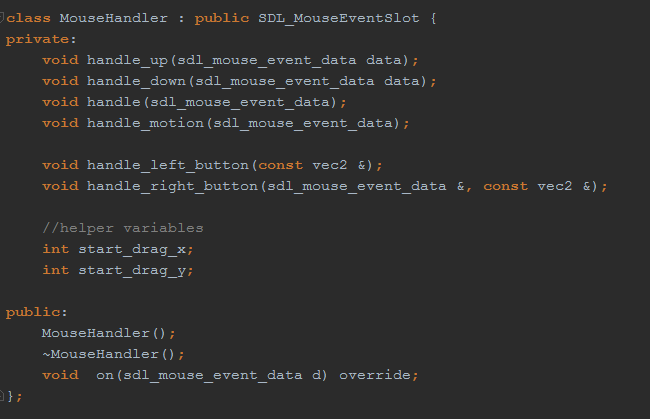
\includegraphics[scale=1.25]{images/MouseHandler.png}
    \caption{MouseHandler class}\label{fig:fuzzy-distance}
\end{figure}

\newpage
The class has a lot of private methods that handle the user input separately. It has one method that has been overridden from the base class, which is the on-method. The on-method is where user inputs comes in. In this method the input is separated into two groups and will be handled further by other methods. To make clear how this works an explanatory activity diagram can be found below to illustrate the process. Below the image we will globally explain what the methods do individually. If 

\begin{figure}[!htb]
    \centering
    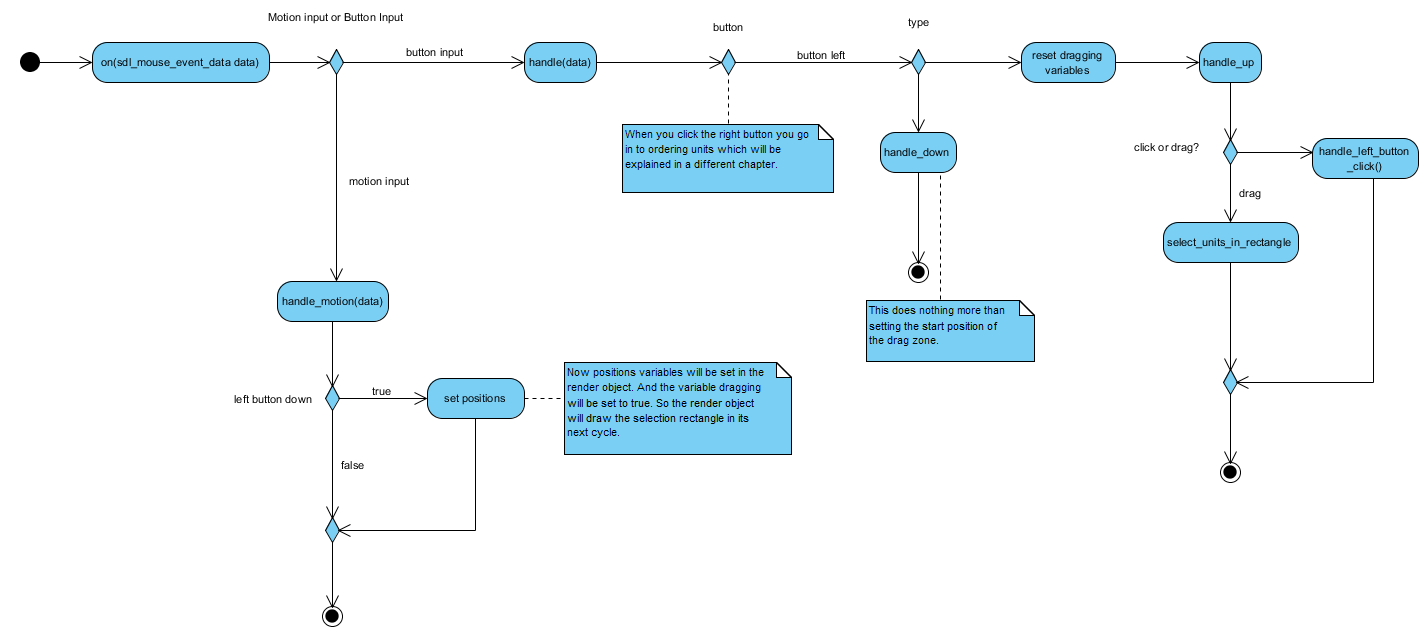
\includegraphics[scale=0.55]{images/ActivityDiagramMouseHandler.PNG}
    \caption{handling user input activity diagram}\label{fig:fuzzy-distance}
\end{figure}
\newpage

If the text in the image is unreadable, we recommend taking a look at the PNG file in the images folder.



\end{abstract}
